\documentclass{article}
\usepackage[utf8]{inputenc}
\usepackage{tikz}
\usetikzlibrary{shadows, shapes.geometric, shapes.symbols,  arrows}

\begin{document}

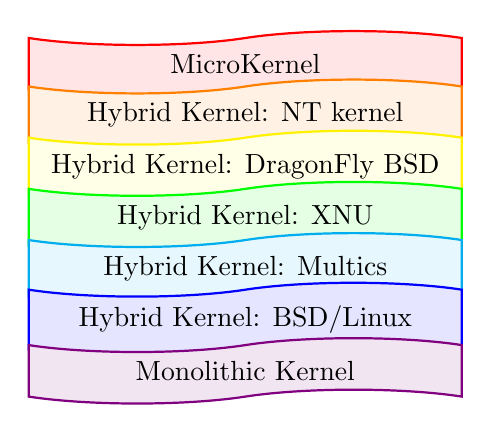
\begin{tikzpicture}[node distance=1mm]

\node at (0, 0) [align=center,tape,minimum  width=5.5cm,draw=red,thick,fill=red!10]
{MicroKernel};
\node at (0, -0.65) [align=center,tape,minimum  width=5.5cm,draw=orange,thick,fill=orange!10]
{Hybrid Kernel: NT kernel};
\node at (0, -1.3)
[align=center,tape,minimum  width=5.5cm,draw=yellow,thick,fill=yellow!10]
{Hybrid Kernel: DragonFly BSD};
\node at (0, -1.95)
[align=center,tape,minimum  width=5.5cm,draw=green,thick,fill=green!10]
{Hybrid Kernel: XNU};
\node at (0, -2.6)
[align=center,tape,minimum  width=5.5cm,draw=cyan,thick,fill=cyan!10]
{Hybrid Kernel: Multics};
\node at (0, -3.25)
[align=center,tape,minimum  width=5.5cm,draw=blue,thick,fill=blue!10]
{Hybrid Kernel: BSD/Linux};
\node at (0, -3.9)
[align=center,tape,minimum  width=5.5cm,draw=violet,thick,fill=violet!10]
{Monolithic Kernel};

\end{tikzpicture}

\end{document}